\documentclass[journal,12pt,onecolumn]{IEEEtran}
\usepackage{cite}
\usepackage{graphicx}
\usepackage{amsmath,amssymb,amsfonts,amsthm}
\usepackage{algorithmic}
\usepackage{graphicx}
\usepackage{textcomp}
\usepackage{xcolor}
\usepackage{txfonts}
\usepackage{listings}
\usepackage{enumitem}
\usepackage{mathtools}
\usepackage{gensymb}
\usepackage{comment}
\usepackage[breaklinks=true]{hyperref}
\usepackage{tkz-euclide} 
\usepackage{listings}
\usepackage{gvv}                                        
\usepackage[latin1]{inputenc} 
\usetikzlibrary{arrows.meta, positioning}
\usepackage{xparse}
\usepackage{color}                                            
\usepackage{array}                                            
\usepackage{longtable}                                       
\usepackage{calc}                                             
\usepackage{multirow}
\usepackage{multicol}
\usepackage{hhline}                                           
\usepackage{ifthen}                                           
\usepackage{lscape}
\usepackage{tabularx}
\usepackage{array}
\usepackage{float}
\newtheorem{theorem}{Theorem}[section]
\newtheorem{problem}{Problem}
\newtheorem{proposition}{Proposition}[section]
\newtheorem{lemma}{Lemma}[section]
\newtheorem{corollary}[theorem]{Corollary}
\newtheorem{example}{Example}[section]
\newtheorem{definition}[problem]{Definition}
\newcommand{\BEQA}{\begin{eqnarray}}
\newcommand{\EEQA}{\end{eqnarray}}
\usepackage{float}
\theoremstyle{remark}
\usepackage{circuitikz}
\usepackage{tikz}
\title{GG2: GEOLOGY AND GEOPHYSICS}
\author{EE25BTECH11032- KARTIK LAHOTI}

\begin{document}
\maketitle

\begin{enumerate}

\item Is there any good show \rule{3cm}{0.15mm} television tonight?
Select the most appropriate option to complete the above sentence. \hfill{\brak{\text{GATE GG-2 2025}}}
\begin{enumerate}
    \begin{multicols}{4}
    \item in
    \item at
    \item within
    \item on
    \end{multicols}
\end{enumerate}

\item As the police officer was found guilty of embezzlement, he was \rule{3cm}{0.15mm} dismissed from the service in accordance with the Service Rules.
Select the most appropriate option to complete the above sentence. \hfill{\brak{\text{GATE GG-2 2025}}}
\begin{enumerate}
    \begin{multicols}{4}
    \item sumptuously
    \item brazenly
    \item unintentionally
    \item summarily
    \end{multicols}
\end{enumerate}

\item The sum of the following infinite series is:
\begin{align*}
\frac{1}{1!} + \frac{1}{2!} + \frac{1}{3!} + \frac{1}{4!} + \frac{1}{5!} + \cdots
\end{align*}
\hfill{\brak{\text{GATE GG-2 2025}}}
\begin{enumerate}
    \begin{multicols}{4}
    \item $\pi$
    \item $1+e$
    \item $e-1$
    \item $e$
    \end{multicols}
\end{enumerate}

\item A thin wire is used to construct all the edges of a cube of $1\,m$ side by bending, cutting and soldering the wire. If the wire is $12\,m$ long, what is the minimum number of cuts required to construct the wire frame to form the cube? \hfill{\brak{\text{GATE GG-2 2025}}}
\begin{enumerate}
    \begin{multicols}{4}
    \item $3$
    \item $4$
    \item $6$
    \item $12$
    \end{multicols}
\end{enumerate}

\item The figures I, II and III are parts of a sequence. Which one of the following options comes next in the sequence at IV?
\begin{figure}[H]
    \centering
    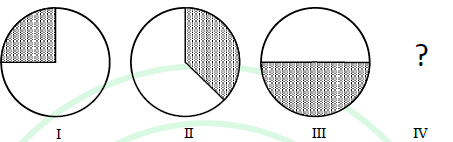
\includegraphics[width=0.8\columnwidth]{figs/fig1.png}
    \caption{}
    \label{fig:q5}
\end{figure}
\hfill{\brak{\text{GATE GG-2 2025}}}
\begin{enumerate}
\begin{multicols}{2}
    \item 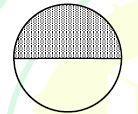
\includegraphics[width=0.2\columnwidth]{figs/fig1a.png} 
    \item 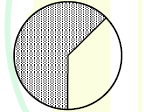
\includegraphics[width=0.2\columnwidth]{figs/fig1b.png} 
    \item 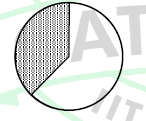
\includegraphics[width=0.2\columnwidth]{figs/fig1c.png} 
    \item 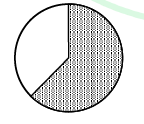
\includegraphics[width=0.2\columnwidth]{figs/fig1d.png}
\end{multicols}
\end{enumerate}

\item "Why do they pull down and do away with crooked streets, I wonder, which are my delight, and hurt no man living? Every day the wealthier nations are pulling down one or another in their capitals and their great towns: they do not know why they do it; neither do I. It ought to be enough, surely, to drive the great broad ways which commerce needs and which are the life-channels of a modern city, without destroying all history and all the humanity in between: the islands of the past." \brak{\text{From Hilaire Belloc's "The Crooked Streets"}}
Based only on the information provided in the above passage, which one of the following statements is true? \hfill{\brak{\text{GATE GG-2 2025}}}
\begin{enumerate}
    \item The author of the passage takes delight in wondering.
    \item The wealthier nations are pulling down the crooked streets in their capitals.
    \item In the past, crooked streets were only built on islands.
    \item Great broad ways are needed to protect commerce and history.
\end{enumerate}

\item Rohit goes to a restaurant for lunch at about $1$ PM. When he enters the restaurant, he notices that the hour and minute hands on the wall clock are exactly coinciding. After about an hour, when he leaves the restaurant, he notices that the clock hands are again exactly coinciding. How much time \brak{\text{in minutes}} did Rohit spend at the restaurant? \hfill{\brak{\text{GATE GG-2 2025}}}
\begin{enumerate}
\begin{multicols}{2}
    \item $64\frac{6}{11}$
    \item $66\frac{5}{13}$
    \item $65\frac{5}{11}$
    \item $66\frac{6}{13}$
    
\end{multicols}    
\end{enumerate}

\item A color model is shown in the figure with color codes: Yellow \brak{Y}, Magenta \brak{M}, Cyan \brak{Cy}, Red \brak{R}, Blue \brak{Bl}, Green \brak{G}, and Black \brak{K}.
\begin{figure}[H]
    \centering
    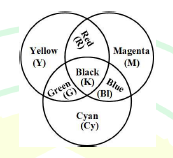
\includegraphics[width=0.5\columnwidth]{figs/fig2.png}
    \caption{}
    \label{fig:q8}
\end{figure}
Which one of the following options displays the color codes that are consistent with the color model? \hfill{\brak{\text{GATE GG-2 2025}}}
\begin{enumerate}
\begin{multicols}{2}
    \item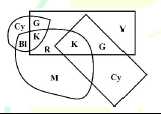
\includegraphics[width=0.4\columnwidth]{figs/fig2a.png}
    \item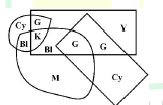
\includegraphics[width=0.4\columnwidth]{figs/fig2b.png}
    \item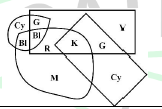
\includegraphics[width=0.4\columnwidth]{figs/fig2c.png}
    \item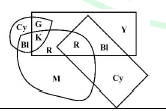
\includegraphics[width=0.4\columnwidth]{figs/fig2d.png}
\end{multicols} 
\end{enumerate}

\item A circle with center at $\brak{x,y}=\brak{0.5,0}$ and radius $=0.5$ intersects with another circle with center at $\brak{x,y}=\brak{1,1}$ and radius $=1$ at two points. One of the points of intersection $\brak{x, y}$ is: \hfill{\brak{\text{GATE GG-2 2025}}}
\begin{enumerate}
    \begin{multicols}{4}
    \item $\brak{0,0}$
    \item $\brak{0.2, 0.4}$
    \item $\brak{0.5, 0.5}$
    \item $\brak{1,2}$
    \end{multicols}
\end{enumerate}

\item An object is said to have an n-fold rotational symmetry if the object, rotated by an angle of $\frac{2\pi}{n}$, is identical to the original. Which one of the following objects exhibits $4$-fold rotational symmetry about an axis perpendicular to the plane of the screen? Note: The figures shown are representative. \hfill{\brak{\text{GATE GG-2 2025}}}
\begin{enumerate}
\begin{multicols}{2}
    \item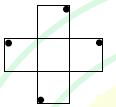
\includegraphics[width=0.4\columnwidth]{figs/fig3a.png}
    \item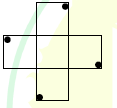
\includegraphics[width=0.4\columnwidth]{figs/fig3b.png}
    \item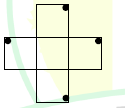
\includegraphics[width=0.4\columnwidth]{figs/fig3c.png}
    \item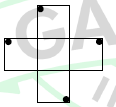
\includegraphics[width=0.4\columnwidth]{figs/fig3d.png}
\end{multicols}
\end{enumerate}

\item The most volcanically active body in our Solar System is  \hfill{\brak{\text{GATE GG-2 2025}}}
\begin{enumerate}
    \begin{multicols}{4}
    \item Mars
    \item Io
    \item Moon
    \item Venus
    \end{multicols}
\end{enumerate}

\item A type of fold which is relatively sharp and angular at its synformal and antiformal hinges is known as  \hfill{\brak{\text{GATE GG-2 2025}}}
\begin{enumerate}
    \begin{multicols}{4}
    \item Drag fold
    \item Chevron fold
    \item Dome
    \item Basin
    \end{multicols}
\end{enumerate}

\item Which one of the following geophysical methods can provide information on deep Earth structures $\brak{\text{of the order of }1000\,km}$ with highest resolution? \hfill{\brak{\text{GATE GG-2 2025}}}
\begin{enumerate}
    \begin{multicols}{2}
    \item Seismic methods
    \item Magnetic methods
    \item Electrical methods
    \item Gravity methods
    \end{multicols}
\end{enumerate}

\item The continuous series of Bowen's reaction series is represented by  \hfill{\brak{\text{GATE GG-2 2025}}}
\begin{enumerate}
    \item the orthoclase - albite feldspar system
    \item the anorthite - albite system
    \item the forsterite - fayalite system
    \item the diopside - anorthite system
\end{enumerate}

\item Which of the following time boundaries correspond\brak{s} to major mass extinction events? \hfill{\brak{\text{GATE GG-2 2025}}}
\begin{enumerate}
    \item Cretaceous - Paleogene
    \item Paleogene - Neogene
    \item Permian Triassic
    \item Precambrian - Cambrian
\end{enumerate}

\item A watershed has an area of $74 \text{ km}^2$. The stream network within this watershed consists of three different stream orders. The stream lengths in each order are as follows: 

$I^{st}$ order streams: $3\,km$ km, $2.5\,km$, $4\,km$, $3\,km$, $2\,km$, $5\,km$ 

$II^{nd}$ order streams: $10\,km$, $15\,km$, $7\,km$ 

$III^{rd}$ order streams: $30\,km$ 

The drainage density of the watershed is \rule{3cm}{0.15mm} $\text{km/km}^2$. \brak{\text{Round off to two decimal places}} \hfill{\brak{\text{GATE GG-2 2025}}}

\item A sample contains $7\, wt\,\%\,CaO$ and $5\, wt\,\%\,MgO$. The molar ratio of $CaO$ to $MgO$ in the sample is \rule{3cm}{0.15mm}. \brak{\text{Round off to two decimal places}} \hfill{\brak{\text{GATE GG-2 2025}}}

\item Select the option that lists oxide minerals only. \hfill{\brak{\text{GATE GG-2 2025}}}
\begin{enumerate}
    \item Spinel, Corundum, Rutile
    \item Olivine, Pyroxene, Magnetite
    \item Apatite, Galena, Monazite
    \item Fluorite, Halite, Calcite
\end{enumerate}

\item Consider two intersecting, north-easterly striking and south-easterly dipping dikes Y1 and Y2, which are exposed on an east-west trending vertical wall of a granite \brak{X} quarry as shown below.
\begin{figure}[H]
    \centering
    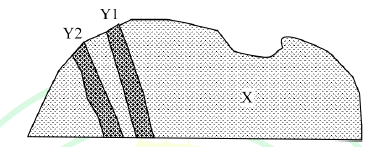
\includegraphics[width=0.5\columnwidth]{figs/fig4.png}
    \caption{}
    \label{fig:q19}
\end{figure}
The angle that the dikes make with the horizontal on the quarry wall is \rule{3cm}{0.15mm} \hfill{\brak{\text{GATE GG-2 2025}}}
\begin{enumerate}
\begin{multicols}{2}
    \item true dip
    \item apparent dip
    \item rake
    \item attitude of foliation
\end{multicols}
\end{enumerate}

\item The ratio of P-wave to S-wave velocities, $V_p/V_s$, within the Earth depends on \rule{3cm}{0.15mm} \hfill{\brak{\text{GATE GG-2 2025}}}
\begin{enumerate}
\begin{multicols}{2}
    \item bulk modulus
    \item shear modulus
    \item density
    \item coefficient of internal friction
\end{multicols}
\end{enumerate}

\item Three pixels P, Q, and R in an image are characterized by the NDVI values of $+0.84$, $+0.01$, and $-0.89$, respectively. Which of the following options is/are correct? \hfill{\brak{\text{GATE GG-2 2025}}}
\begin{enumerate}
    \item P is from vegetation area and Q is from barren land
    \item Q is from water body and R is from barren land
    \item Q is from barren land and R is from water body
    \item P is from vegetation area and Q is from water body
\end{enumerate}

\item Which of the following can indicate the presence of significant sub-surface iron mineralization? \hfill{\brak{\text{GATE GG-2 2025}}}
\begin{enumerate}
    \item Free air gravity anomaly
    \item Bouguer gravity anomaly
    \item Magnetic anomaly
    \item Electrical resistivity measurements
\end{enumerate}

\item Which of the following statements is/are correct regarding the magnetic field lines of the Earth, at the magnetic poles and the magnetic equator? \hfill{\brak{\text{GATE GG-2 2025}}}
\begin{enumerate}
    \item Horizonal at the equator
    \item Vertical at the poles
    \item Horizonal at the poles
    \item Vertical at the equator
\end{enumerate}

\item If the lowest Digital Number \brak{DN} value in an image of $10$-bit radiometric resolution is $0$, then the maximum DN value of that image is \rule{3cm}{0.15mm}. \brak{\text{Answer in integer}} \hfill{\brak{\text{GATE GG-2 2025}}}

\item If one liter of water at pH $7$ is mixed with one liter of water at pH $6$, the resulting pH of the mixture is \rule{3cm}{0.15mm}. \brak{\text{Round off to two decimal places}} \hfill{\brak{\text{GATE GG-2 2025}}}

\item A hillslope is shown below. If the area over the failure plane is $50 \text{ m}^2$ and the weight of the hillslope material \brak{W} is $2000$ tons, the Factor of Safety \brak{FOS} for this hillslope in dry conditions is \rule{3cm}{0.15mm}. \brak{\text{Cohesion along failure plane $=196$ KPa, dip of failure plane $=60\degree$, and internal friction angle $=30\degree$}}. \brak{\text{Round off to two decimal places}}
\begin{figure}[H]
    \centering
    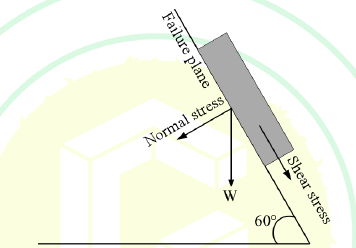
\includegraphics[width=0.5\columnwidth]{figs/fig5.png}
    \caption{}
    \label{fig:q26}
\end{figure}
\hfill{\brak{\text{GATE GG-2 2025}}}

% Question 27
\item A scalar potential $\psi$ of a vector field, F, satisfies the Laplace equation $\brak{\nabla^2 \psi = 0}$ in free space. $\psi$ can be uniquely determined at any point inside the closed surface S using  \hfill{\brak{\text{GATE GG-2 2025}}}
\begin{enumerate}
\begin{multicols}{4}
    \item $\nabla \cdot F = 0$
    \item $\nabla \times F = 0$
    \item $\psi\brak{x} = \text{constant}, x \in S$
    \item $\nabla \cdot F \ne 0$
\end{multicols}
\end{enumerate}

% Question 28
\item In resistivity measurements for a double-dipole system, the apparent resistivity is NOT affected by \hfill{\brak{\text{GATE GG-2 2025}}}
\begin{enumerate}
    \item the electrode spacing
    \item the resistivity of the subsurface
    \item the distance between the centers of the current and potential dipoles
    \item the telluric current
\end{enumerate}

% Question 29
\item The working of the proton-precession magnetometer is based on \hfill{\brak{\text{GATE GG-2 2025}}}
\begin{enumerate}
    \item the magnetic moment of hydrogen-atom nucleus being proportional to the angular momentum of its spin
    \item the fact that oxygen is diamagnetic
    \item the fact that the lowest energy level of electrons is in the ground state
    \item the Zeeman effect
\end{enumerate}

% Question 30
\item Which one of these statements is NOT correct for electromagnetic waves travelling through the subsurface? \hfill{\brak{\text{GATE GG-2 2025}}}
\begin{enumerate}
    \item They cannot travel without attenuation
    \item They are subject to diffraction
    \item They are analogous to seismic P waves
    \item They can be used to detect highly conductive ore bodies
\end{enumerate}

% Question 31
\item Diurnal correction in magnetic survey data accounts for  \hfill{\brak{\text{GATE GG-2 2025}}}
\begin{enumerate}
    \item geomagnetic polarity reversals
    \item charged particles in ionosphere
    \item the westward drift of the Earth's magnetic field
    \item the lunar magnetic field
\end{enumerate}

% Question 32
\item Which one of the following options is the primary contributor to the International Geomagnetic Reference Field? \hfill{\brak{\text{GATE GG-2 2025}}}
\begin{enumerate}
    \item Ionospheric magnetic field
    \item Magnetic field generated in the outer core
    \item Crustal magnetic field
    \item Solar magnetic field
\end{enumerate}

% Question 33
\item If a planet is made of uniform density material and has no topography, then which one of the following statements is correct? \hfill{\brak{\text{GATE GG-2 2025}}}
\begin{enumerate}
    \item The geoid surface would be higher than the reference ellipsoid surface
    \item The geoid surface would be lower than the reference ellipsoid surface
    \item The geoid and the reference ellipsoid surfaces would coincide
    \item The geoid surface would be lower in some places, and higher in other places, with respect to the reference ellipsoid
\end{enumerate}

% Question 34
\item Which one of the following factors leads to an abrupt increase in density at the mantle-outer core boundary? \hfill{\brak{\text{GATE GG-2 2025}}}
\begin{enumerate}
\begin{multicols}{4}   
    \item Composition change
    \item Temperature change
    \item Phase change
    \item Viscosity change
\end{multicols}
\end{enumerate}

% Question 35
\item Which one of the options is correct about $\beta^-$ decay? \hfill{\brak{\text{GATE GG-2 2025}}}
\begin{enumerate}
    \item Atomic number increases and mass number remains constant
    \item Atomic weight increases and atomic number remains constant
    \item Number of protons increases and number of neutrons remains constant
    \item Number of neutrons increases and number of protons remains constant
\end{enumerate}

% Question 36
\item F denotes force, A denotes area, L denotes length, and $\Delta$L is the change in length due to the applied force. Assuming linear elasticity, select a relationship where the constant of proportionality is a material property independent of the dimensions of the body. \hfill{\brak{\text{GATE GG-2 2025}}}
\begin{enumerate}
    \item $F \propto \Delta L$
    \item $F \propto \Delta L/L$
    \item $F \propto A \times \Delta L/L$
    \item $F \propto \Delta L \times L/A$
\end{enumerate}

% Question 37
\item In a gravity survey that is being carried out in the vicinity of a large mountain, it was observed that the deflection of the plumb line from the vertical is less than what is calculated using the visible mountain mass. Which one of the inferences about the mountain is correct? \hfill{\brak{\text{GATE GG-2 2025}}}
\begin{enumerate}
    \item It has a high-density root
    \item It has no root
    \item It has a low-density root
    \item It has a high-density anti-root
\end{enumerate}

% Question 38
\item In the schematic, line P shows a $1$-D geothermal profile. If the heat flow at the base of the mantle increases, which line will reflect the new geothermal profile?
\begin{figure}[H]
    \centering
    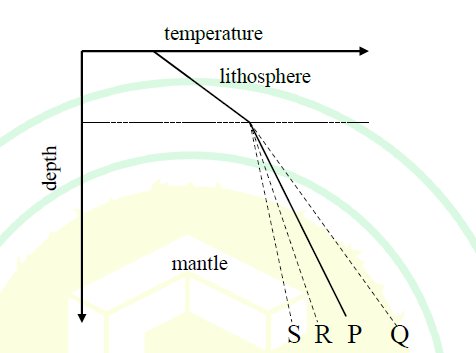
\includegraphics[width=0.6\columnwidth]{figs/fig6.png}
    \caption{}
    \label{fig:q38}
\end{figure}
\hfill{\brak{\text{GATE GG-2 2025}}}
\begin{enumerate}
\begin{multicols}{4}
    \item Line Q
    \item Line R
    \item Line S
    \item Line P
\end{multicols}
\end{enumerate}

% Question 39
\item The following figure shows the GPS data at two stations located near each other at the same latitude. Station A is moving towards the west while station B is moving towards the east. Which one of the following options is correct?
\begin{figure}[H]
    \centering
    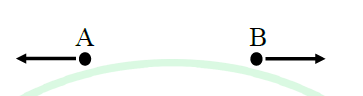
\includegraphics[width=0.5\columnwidth]{figs/fig7.png}
    \caption{}
    \label{fig:q39}
\end{figure}
\hfill{\brak{\text{GATE GG-2 2025}}}
\begin{enumerate}
    \item A and B are located on two sides of a convergent boundary
    \item A and B are located on two sides of a transform boundary
    \item A and B are located on two sides of a divergent boundary
    \item A and B are parts of the same plate
\end{enumerate}

% Question 40
\item The following figure shows a region in which rocks in areas A, B and C follow Hooke's law and are subject to the same stress. B exhibits lower strain than both A and C. What can we infer about the nature of B?
\begin{figure}[H]
    \centering
    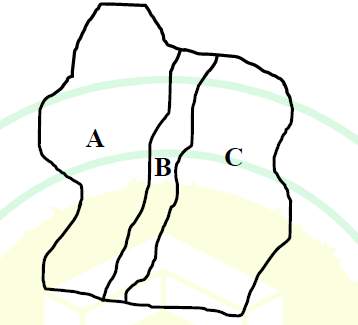
\includegraphics[width=0.5\columnwidth]{figs/fig8.png}
    \caption{}
    \label{fig:q40}
\end{figure}
\hfill{\brak{\text{GATE GG-2 2025}}}
\begin{enumerate}
    \item B is part of a plate boundary
    \item B has higher heat flow values compared to A and C
    \item B is made up of rocks of lower density compared to A and C
    \item B is made up of rocks that have higher strength compared to A and C
\end{enumerate}

% Question 41
\item What is/are the primary effect\brak{s} of applying upward continuation to magnetic field data? \hfill{\brak{\text{GATE GG-2 2025}}}
\begin{enumerate}
    \item Decrease in the relative influence of shallow magnetic sources
    \item Increase in the relative influence of deeper magnetic sources
    \item Improvement in the detection of near-surface magnetic sources
    \item Movement of shallow magnetic sources closer to the observation plane
\end{enumerate}

% Question 42
\item Half-life of $^{14}C$ is $5730$ years. Suppose we start with $1$ billon $^{14}C$ atoms and after a certain interval of time only $125$ million $^{14}C$ atoms remain, the number of half-lives that has elapsed is \rule{3cm}{0.15mm}. \brak{\text{Answer in integer}} \hfill{\brak{\text{GATE GG-2 2025}}}

% Question 43
\item When an external magnetic field of strength $1.5 \times 10^{-3}\,A/m$ is applied to a rock sample, the measured intensity of magnetization is $0.5 \times 10^{-3}\,A/m$. The magnetic susceptibility of this rock is \rule{3cm}{0.15mm}. \brak{\text{Round off to two decimal places}} \hfill{\brak{\text{GATE GG-2 2025}}}

% Question 44
\item If seismic signals of periods greater than $10$ s are of interest, the minimum sampling frequency should be \rule{3cm}{0.15mm} $Hz$. \brak{\text{Round off to one decimal place}} \hfill{\brak{\text{GATE GG-2 2025}}}

% Question 45
\item The components $ u, v, w$ of the displacement field along $x, y, z$ directions, respectively, are given by
\begin{align*}
u &= -\sin\brak{\omega t - kz} \\
v &= \sin\brak{\omega t - kz} \\
w &= 0
\end{align*}
where, $t$, $k$, and $\omega$ are time, wavenumber, and angular frequency, respectively. Assuming $k$ is real, which one of the following options describes the wave? \hfill{\brak{\text{GATE GG-2 2025}}}
\begin{enumerate}
    \item An S-wave propagating in the $z$ direction
    \item A P-wave propagating in the $z$ direction
    \item A Rayleigh wave with elliptical motion in the $xy$ plane
    \item An S-wave travelling in the $x$ direction
\end{enumerate}

% Question 46
\item Select the correct statement regarding surface waves and upper mantle structure. \hfill{\brak{\text{GATE GG-2 2025}}}
\begin{enumerate}
    \item Surface waves cannot be used to infer the upper mantle structure as the amplitudes decay with increasing distance from the surface
    \item Surface waves can be used to infer the upper mantle structure as surface wave phase velocity varies with frequency
    \item Surface waves can be used to infer the upper mantle structure as the shear-wave velocity of the medium changes with frequency
    \item Surface waves cannot be used to infer the upper mantle structure as surface waves travel only along the surface and are not sensitive to the Earth's internal structure
\end{enumerate}

% Question 47
\item A geophysicist is analyzing the elastic-wave radiation to infer the body force equivalent of a seismic source. She has plotted the horizontal component of the displacement field, denoted as $u\brak{m,t}$, for time t and location m. The measured field at two locations m and n is plotted in the figure. Note that S and P waves have negligible amplitudes at locations m and n, respectively. Assuming a homogeneous medium, select the most probable direction $\brak{\text{specified by the angle} \alpha}$ along which the force $\vec{F}$ is applied.
\begin{figure}[H]
    \centering
    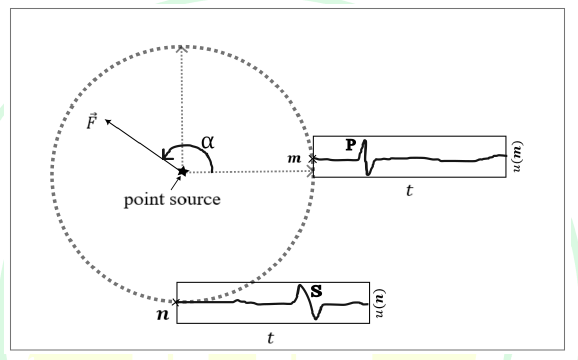
\includegraphics[width=0.7\columnwidth]{figs/fig9.png}
    \caption{}
    \label{fig:q47}
\end{figure}
\hfill{\brak{\text{GATE GG-2 2025}}}
\begin{enumerate}
\begin{multicols}{4}
    \item $\alpha = 0\degree$
    \item $\alpha = 90\degree$
    \item $\alpha = 135\degree$
    \item $\alpha = 315\degree$
\end{multicols}
\end{enumerate}

% Question 48
\item For a horizontal liquid-solid interface as shown, which one of the following ray diagrams with an incident P wave is correct? SH and SV denote shear-horizontal and shear-vertical waves, respectively.
\begin{figure}[H]
    \centering
    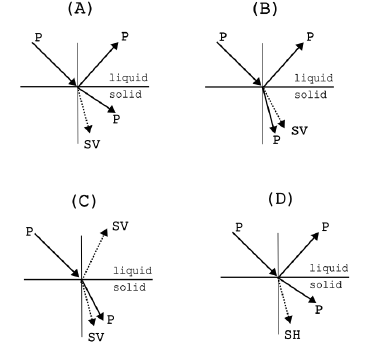
\includegraphics[width=0.7\columnwidth]{figs/fig16.png}
    \caption{}
    \label{fig:q48}
\end{figure}
\hfill{\brak{\text{GATE GG-2 2025}}}
\begin{enumerate}
\begin{multicols}{4}
    \item A
    \item B
    \item C
    \item D
\end{multicols}
\end{enumerate}

% Question 49
\item Consider a steady state heat conduction equation for the Earth's crust where A is the heat source and $k$ is the thermal conductivity. Given the boundary conditions: 

$i$) $T=0$ at the surface and 

$ii$) Q is the heat flux at the surface, 

which one of the following options would be the temperature $\brak{T}$ at depth $z$? \hfill{\brak{\text{GATE GG-2 2025}}}
\begin{enumerate}
    \item $-\frac{\brak{Az+2Q}z}{2k}$
    \item $-\frac{\brak{Az+2Q}z}{k}$
    \item $-\frac{\brak{Az+Q}z}{2k}$
    \item $-\frac{\brak{A+2Q}z^2}{2k}$
\end{enumerate}

% Question 50
\item Consider a ray tomography experiment, where the goal is to estimate the wave velocity of $9$ square cells plotted in each of the cases A and B. The ray paths for source-receiver pairs for both these cases are shown in the figure. Select the correct statement.
\begin{figure}[H]
    \centering
    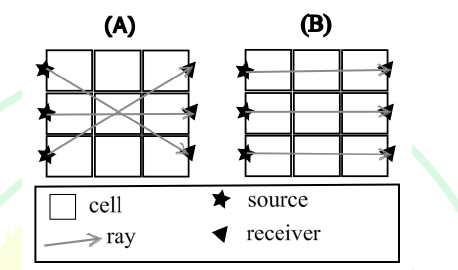
\includegraphics[width=0.6\columnwidth]{figs/fig10.png}
    \caption{}
    \label{fig:q50}
\end{figure}
\hfill{\brak{\text{GATE GG-2 2025}}}
\begin{enumerate}
    \item Both A and B are well-determined problems
    \item Case A has a unique solution, and B is underdetermined
    \item Both A and B are mixed determined problems
    \item Case A is mixed determined, and B is underdetermined
\end{enumerate}

% Question 51
\item Consider extracting the subsurface medium response by cross-correlating seismic ambient noise $u\brak{t}$ and $v\brak{t}$ measured at two stations. The cross-correlation $x\brak{t} = \Sigma_{\tau} u\brak{\tau}v\brak{\tau+t}$ averaged over a period of one year is plotted in the figure, with most of the energy in the positive time lags. In this figure, four probable seismic sources are marked \brak{i}, \brak{ii}, \brak{iii} and \brak{iv}. Assuming a homogeneous medium, select the source that is most probably excited.
\begin{figure}[H]
    \centering
    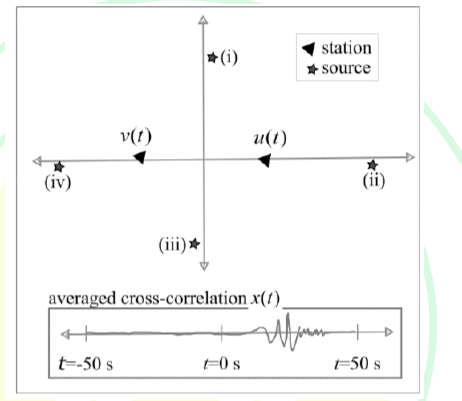
\includegraphics[width=0.7\columnwidth]{figs/fig11.png}
    \caption{}
    \label{fig:q51}
\end{figure}
\hfill{\brak{\text{GATE GG-2 2025}}}
\begin{enumerate}
\begin{multicols}{4}
    \item \brak{i}
    \item \brak{ii}
    \item \brak{iii}
    \item \brak{iv}
\end{multicols}
\end{enumerate}

% Question 52
\item Given the following electric field in cartesian coordinates
\begin{align*}
    E = x^2y\hat{i} + y^2z\hat{j} + z^2x\hat{k},
\end{align*}
which of the following statements is/are correct? \hfill{\brak{\text{GATE GG-2 2025}}}
\begin{enumerate}
    \item The electric field is not conservative
    \item The electric field is static
    \item Both divergence and curl of the electric field are zero
    \item Electric field is neither conservative nor static
\end{enumerate}

% Question 53
\item What factor\brak{s} determine\brak{s} the magnitude of peak ground acceleration measured at a particular station due to an earthquake? \hfill{\brak{\text{GATE GG-2 2025}}}
\begin{enumerate}
\begin{multicols}{2}
    \item Distance from the earthquake
    \item Rupture directivity
    \item Origin time of the earthquake
    \item Type of soil
\end{multicols}
\end{enumerate}

% Question 54
\item Consider a geophysical inverse problem of the form $d=Gm$, where $G$ is the forward operator, $m$ is the model vector and $d$ is the observed data vector. The Earth model parameters can be estimated using $m^{\text{est}}=Hd$, where $H$ is the pseudoinverse of $G$. Given $G=U\Sigma V^T$ as the singular value decomposition of $G$, and assuming $G$ is full rank, which of the following options is/are correct? \hfill{\brak{\text{GATE GG-2 2025}}}
\begin{enumerate}
\begin{multicols}{4}
    \item $H=U^T\Sigma^{-1}V$
    \item $H=V\Sigma^{-1}U^T$
    \item $H=U^T\Sigma^{-1}V^T$
    \item $H=UU^TV\Sigma^{-1}U^T$
    \end{multicols}
\end{enumerate}

% Question 55
\item Consider ray tracing in an isotropic elastic Earth, with travel time function $T\brak{x,y,z}$ in Cartesian coordinates. Select the correct option\brak{s}. \hfill{\brak{\text{GATE GG-2 2025}}}
\begin{enumerate}
    \item The slowness vector is tangential to the wave fronts
    \item The slowness vector is parallel to the gradient of $T\brak{x,y,z}$
    \item $T\brak{x,y,z}$ is constant on a particular wave front
    \item $T\brak{x,y,z}$ is constant along the rays
\end{enumerate}

% Question 56
\item Which of the following statements is/are correct regarding the properties of the oceanic lithosphere? \hfill{\brak{\text{GATE GG-2 2025}}}
\begin{enumerate}
    \item Older lithosphere cools at a slower rate compared to younger lithosphere
    \item Heat flow increases with lithospheric age
    \item Heat flow in the lithosphere increases with distance from the spreading ridge
    \item Thickness of the lithosphere increases with age
\end{enumerate}

% Question 57
\item For a half space composed of $3$ layers with resistivities $\rho_1$, $\rho_2$ and $\rho_3$, as shown in the figure, which of the following statements is/are correct about the variation of apparent resistivity with electrode spacing?
\begin{figure}[H]
    \centering
    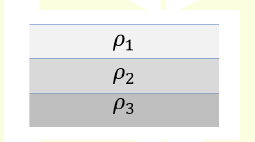
\includegraphics[width=0.3\columnwidth]{figs/fig12.png}
    \caption{}
    \label{fig:q57}
\end{figure}
\hfill{\brak{\text{GATE GG-2 2025}}}
\begin{enumerate}
    \item If $\rho_1 < \rho_2 < \rho_3$, the curve of apparent resistivity increases monotonically
    \item If $\rho_1 < \rho_2 > \rho_3$, the curve of apparent resistivity decreases monotonically
    \item If $\rho_1 > \rho_2 < \rho_3$, the curve of apparent resistivity first decreases and then increases
    \item If $\rho_1 > \rho_2 > \rho_3$, the curve of apparent resistivity increases monotonically
\end{enumerate}

% Question 58
\item A loop of radius R carries a current I and produces a magnetic field B. Which of the following statements is/are correct about B? \hfill{\brak{\text{GATE GG-2 2025}}}
\begin{enumerate}
    \item The magnitude of B is directly proportional to I
    \item The magnitude of B is inversely proportional to the square of radius R
    \item The direction of B is perpendicular to the plane of the loop
    \item The direction of B is parallel to the plane of the loop
\end{enumerate}

% Question 59
\item In seismology, Born approximation of the scattered \brak{perturbed} wavefield is given by
\begin{align*}
    \delta u\brak{r,s;t} \approx \int_V \delta r\brak{x}\brak{u_0\brak{x,s;t} *_t u_0\brak{r,x;t}}dx
\end{align*}
Here, $*_t$ denotes temporal convolution, $\delta r\brak{x}$ is the strength of the scatterer at $x$ in volume $V$, $\delta u\brak{r,s;t}$ is the scattered wavefield measured at the receiver $r$ from the source $s$, $u_0\brak{x,s;t}$ is the downgoing wavefield \brak{to the scatterer at x from the source s} in the unperturbed medium, $u_0\brak{r,x;t}$ is the upgoing wavefield \brak{to the receiver r from the scatterer at x} in the unperturbed medium. Select the correct statement\brak{s}. \hfill{\brak{\text{GATE GG-2 2025}}}
\begin{enumerate}
    \item The Born approximation can be used to model multiply scattered waves
    \item The Born approximation can model only first-order scattering
    \item The scattered wavefield varies linearly with strength of the scatterers
    \item The Born approximation can be used to model head waves from a horizontal reflector
\end{enumerate}

% Question 60
\item A primary electromagnetic field $\brak{H_P}$ is being generated from current $I_P$ flowing in a coil A with negligible capacitance, such that $H_P = KI_P \sin\brak{\omega t}$, where $\omega$ is the angular frequency, $K$ is a constant and $t$ is time. A secondary electromagnetic field is being produced by induction in a conducting coil B. The phase difference between the primary and the secondary electromagnetic fields depends on which of the following factors? \hfill{\brak{\text{GATE GG-2 2025}}}
\begin{enumerate}
    \item Inductance of coil B
    \item Resistance of coil B
    \item Frequency of the primary electromagnetic field
    \item Total current $\brak{I_P}$ flowing through the coil A
\end{enumerate}

% Question 61
\item Consider a medium of uniform resistivity with a pair of source and sink electrodes separated by a distance L, as shown in the figure. The fraction of the input current \brak{I} that flows horizontally $\brak{I_x}$ across the median plane between depths $Z_1 = \frac{L}{2}$ and $Z_2 = \frac{L\sqrt{3}}{2}$, is given by $\frac{I_x}{I} = \frac{L}{\pi} \int_{Z_1}^{Z_2} \frac{dz}{\brak{\frac{L^2}{4} + z^2}}$. The value of $\frac{I_x}{I}$ is equal to \rule{3cm}{0.15mm}. \brak{\text{round off to two decimal places}}
\begin{figure}[H]
    \centering
    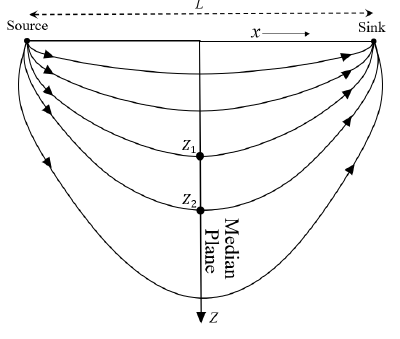
\includegraphics[width=0.6\columnwidth]{figs/fig13.png}
    \caption{}
    \label{fig:q61}
\end{figure}
\hfill{\brak{\text{GATE GG-2 2025}}}

% Question 62
\item Suppose a mountain at location A is in isostatic equilibrium with a column at location B, which is at sea-level, as shown in the figure. The height of the mountain is $4\,km$ and the thickness of the crust at B is $1\,km$. Given the densities of crust and mantle are $2700\,kg/m^3$ and $3300 \,kg/m^3$, respectively, the thickness of the mountain root \brak{r1} is \rule{3cm}{0.15mm} $km$. \brak{\text{Answer in integer}}
\begin{figure}[H]
    \centering
    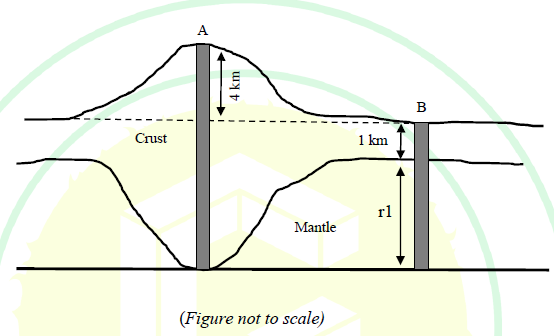
\includegraphics[width=0.7\columnwidth]{figs/fig14.png}
    \caption{}
    \label{fig:q62}
\end{figure}
\hfill{\brak{\text{GATE GG-2 2025}}}

% Question 63
\item While doing Bayesian inference, consider estimating the posterior distribution of the model parameter \brak{m}, given data \brak{d}. Assume that Prior and Likelihood are proportional to Gaussian functions given by
\begin{align*}
\text{Prior} &\propto \exp\brak{-0.5\brak{m-1}^2} \\
\text{Likelihood} &\propto \exp\brak{-0.5\brak{m-3}^2}
\end{align*}
\begin{figure}[H]
    \centering
    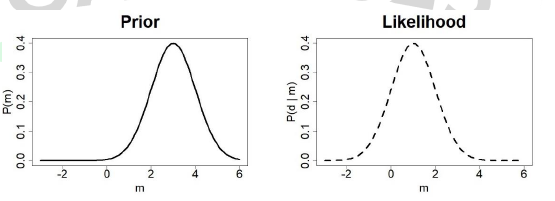
\includegraphics[width=0.8\columnwidth]{figs/fig15.png}
    \caption{}
    \label{fig:q63}
\end{figure}
The mean of the posterior distribution is \rule{3cm}{0.15mm}. \brak{\text{Answer in integer}} \hfill{\brak{\text{GATE GG-2 2025}}}

% Question 64
\item Consider a two-dimensional reflection experiment, where a horizontal boundary between two layers is at a depth of $500\,m$ below the free surface. A source and geophone are placed on the free surface with an offset of $2000\,m$. The P wave velocity of the top layer is $3000 \,m/s$. The travel time of a recorded free-surface reflection multiple, which got reflected twice at the free surface, is \rule{3cm}{0.15mm} $s$. \brak{\text{Round off to two decimal places}} \hfill{\brak{\text{GATE GG-2 2025}}}

% Question 65
\item Consider the acceleration due to gravity $\brak{g'}$ at an altitude $\brak{h} $ of $50\,km$ above the Earth's surface. If $R$ is the radius of the Earth, and the acceleration due to gravity measured at the surface is $g$, the ratio of $g' \text{ to } g$, is \rule{3cm}{0.15mm}. \brak{\text{Assume $h \ll R$, $R=6370\,km$ , and round off to two decimal places}} \hfill{\brak{\text{GATE GG-2 2025}}}

\end{enumerate}


\end{document}
